%me=0 student solutions (ps file), me=1 - my solutions (sol file), me=2 - assignment (hw file)
\def\me{0}
\def\num{5}  %homework number
\def\due{Tuesday, October 13}  %due date
\def\course{CSCI-GA.1170-001/002 Fundamental Algorithms} %course name, changed only once
\def\name{GOWTHAM GOLI (N17656180)}   %student changes (instructor keeps!)
%
\iffalse
INSTRUCTIONS: replace # by the homework number.
(if this is not ps#.tex, use the right file name)

  Clip out the ********* INSERT HERE ********* bits below and insert
appropriate TeX code.  Once you are done with your file, run

  ``latex ps#.tex''

from a UNIX prompt.  If your LaTeX code is clean, the latex will exit
back to a prompt.  To see intermediate results, type

  ``xdvi ps#.dvi'' (from UNIX prompt)
  ``yap ps#.dvi'' (if using MikTex in Windows)

after compilation. Once you are done, run

  ``dvips ps#.dvi''

which should print your file to the nearest printer.  There will be
residual files called ps#.log, ps#.aux, and ps#.dvi.  All these can be
deleted, but do not delete ps1.tex. To generate postscript file ps#.ps,
run

  ``dvips -o ps#.ps ps#.dvi''

I assume you know how to print .ps files (``lpr -Pprinter ps#.ps'')
\fi
%
\documentclass[11pt]{article}
\usepackage{amsfonts}
\usepackage{latexsym}
\usepackage[lined,boxed,linesnumbered]{algorithm2e}
\usepackage{amsmath}
\usepackage{amsthm}
\usepackage{array}
\usepackage{amssymb}
\usepackage{amsthm}
\usepackage{epsfig}
\usepackage{psfrag}
\usepackage{color}
\usepackage{tikz}
\usepackage{enumerate}
\usetikzlibrary{calc,trees,positioning,arrows,fit,shapes,calc}
\usetikzlibrary{trees}
\usepackage{mathtools}
\usepackage{float}
\setlength{\oddsidemargin}{.0in}
\setlength{\evensidemargin}{.0in}
\setlength{\textwidth}{6.5in}
\setlength{\topmargin}{-0.4in}
\setlength{\textheight}{8.5in}

\newcommand{\handout}[5]{
   \renewcommand{\thepage}{#1, Page \arabic{page}}
   \noindent
   \begin{center}
   \framebox{
      \vbox{
    \hbox to 5.78in { {\bf \course} \hfill #2 }
       \vspace{4mm}
       \hbox to 5.78in { {\Large \hfill #5  \hfill} }
       \vspace{2mm}
       \hbox to 5.78in { {\it #3 \hfill #4} }
      }
   }
   \end{center}
   \vspace*{4mm}
}

\newcounter{pppp}
\newcommand{\prob}{\arabic{pppp}}  %problem number
\newcommand{\increase}{\addtocounter{pppp}{1}}  %problem number

%first argument desription, second number of points
\newcommand{\newproblem}[2]{
\ifnum\me=0
\ifnum\prob>0 \newpage \fi
\increase
\setcounter{page}{1}
\handout{\name, Homework \num, Problem \arabic{pppp}}{\today}{Name: \name}{Due:
\due}{Solutions to Problem \prob\ of Homework \num\ (#2)}
\else
\increase
\section*{Problem \num-\prob~(#1) \hfill {#2}}
\fi
}

%\newcommand{\newproblem}[2]{\increase
%\section*{Problem \num-\prob~(#1) \hfill {#2}}
%}

\def\squarebox#1{\hbox to #1{\hfill\vbox to #1{\vfill}}}
\def\qed{\hspace*{\fill}
        \vbox{\hrule\hbox{\vrule\squarebox{.667em}\vrule}\hrule}}
\newenvironment{solution}{\begin{trivlist}\item[]{\bf Solution:}}
                      {\qed \end{trivlist}}
\newenvironment{solsketch}{\begin{trivlist}\item[]{\bf Solution Sketch:}}
                      {\qed \end{trivlist}}
\newenvironment{code}{\begin{tabbing}
12345\=12345\=12345\=12345\=12345\=12345\=12345\=12345\= \kill }
{\end{tabbing}}

%%%%%\newcommand{\eqref}[1]{Equation~(\ref{eq:#1})}

\newcommand{\hint}[1]{({\bf Hint}: {#1})}
%Put more macros here, as needed.
\newcommand{\room}{\medskip\ni}
\newcommand{\brak}[1]{\langle #1 \rangle}
\newcommand{\bit}[1]{\{0,1\}^{#1}}
\newcommand{\zo}{\{0,1\}}
\newcommand{\C}{{\cal C}}

\newcommand{\nin}{\not\in}
\newcommand{\set}[1]{\{#1\}}
\renewcommand{\ni}{\noindent}
\renewcommand{\gets}{\leftarrow}
\renewcommand{\to}{\rightarrow}
\newcommand{\assign}{:=}
\newcommand{\cT}{\mathcal{T}}

\newcommand{\AND}{\wedge}
\newcommand{\OR}{\vee}

\newcommand{\Forr}{\mbox{\bf For }}
\newcommand{\To}{\mbox{\bf to }}
\newcommand{\Do}{\mbox{\bf Do }}
\newcommand{\Ifi}{\mbox{\bf If }}
\newcommand{\Then}{\mbox{\bf Then }}
\newcommand{\Elsee}{\mbox{\bf Else }}
\newcommand{\Whilee}{\mbox{\bf While }}
\newcommand{\Repeatt}{\mbox{\bf Repeat }}
\newcommand{\Until}{\mbox{\bf Until }}
\newcommand{\Returnn}{\mbox{\bf Return }}
\newcommand{\Swap}{\mbox{\bf Swap }}

\begin{document}

\ifnum\me=0
%\handout{PS\num}{\today}{Name: **** INSERT YOU NAME HERE ****}{Due:
%\due}{Solutions to Problem Set \num}
%
%I collaborated with *********** INSERT COLLABORATORS HERE (INDICATING
%SPECIFIC PROBLEMS) *************.
\fi
\ifnum\me=1
\handout{PS\num}{\today}{Name: Yevgeniy Dodis}{Due: \due}{Solution
{\em Sketches} to Problem Set \num}
\fi
\ifnum\me=2
\handout{PS\num}{\today}{Lecturer: Yevgeniy Dodis}{Due: \due}{Problem
Set \num}
\fi


\newproblem{Dealing with Repetitions}{15 points} 

Assume you are given a data structure $D$ which supports the following
two operations:

\begin{itemize}
\item {\sc Insert}$(D,value)$. Inserts a value $value$ into $D$. If $D$
has $n$ elements, assume this procedure takes $I(n)$ time.
\item {\sc Search}$(D,value)$. It $D$ contains at least one element
equal to $value$, return the pointer to this element (else returns
$nil$). Assume this procedure takes $S(n)$ time.
\item {\sc InOrderWalk}$(D)$. Outputs all $n$ elements of $D$ in
sorted order. Assume this procedure takes linear time $O(n)$.
\end{itemize}

Using $D$, you would like to build a new data structure $R$, which can
deal with many repeated elements more efficiently, by supporting the
following operations.

\begin{itemize}
\item {\sc Add}$(R,value)$. Inserts a value $value$ into $R$. 
\item {\sc Frequency}$(R,value)$. Returns the number of elements of $R$
equal to $value$ (i.e., how many times was {\sc Add}$(R,value)$ called
before).
\item {\sc FastInOrderWalk}$(R)$. Outputs all {\em distinct} 
elements of $D$ in sorted order, together with their frequency values.
\end{itemize}

\begin{itemize}
 \item[(a)] (5 pts) Using $D$, show how to implement $R$, so that the
 following is true. If $R$ contains $n$ records, but only $t$ of them
 are distinct, where $t$ could be much less than $n$, then 

\begin{itemize}
\item {\sc  Add}$(R,key)$ should run in time $A(n,t) \approx I(t) +
 S(t)$;
\item {\sc  Frequency}$(R,key)$ should run in time $F(n,t) \approx
S(t)$;
\item {\sc FastInOrderWalk}$(R)$ should run in time $O(t)$. 
\end{itemize}

Namely, all run times are {\em independent of $n$}.  For example, if
{\sc Add} has been called $4$ times on $(R,7)$ and $5$ times on
$(R,6)$ then {\sc Frequency}$(R,3)$ returns $0$ but {\sc
Frequency}$(R,7)$ returns $4$, and both calls take time $F(9,2)
\approx S(2)$, where $t = 2$ because only two distinct values 
were inserted so far (despite $n=4+5=9$). Also, 
 {\sc FastInOrderWalk}$(R)$ will output $(6,5),(7,4)$ in time $O(2)$.
\\
\hint{Add a field $v.num$ in addition to $v.key$, which counts how
 many elements are equal to $v.key$.}

\ifnum\me<2
\begin{solution}
\section*{Implementing \textit{R} using \textit{D}}
Maintain a field called \textit{num} for each node in $D$ which maintains the frequency of that node and eliminate all the other duplicates from $D$. This new data structure formed is $R$ (i.e $R$ is similar to $D$, the only difference is $R$ has all distinct elements in it and maintains an additional frequency field). Therefore if $D$ has $t$ distinct elements in it then number of elements in $R$ is $t$. 

{\sc Insert}($R, value$) takes $I(t)$ time\\
{\sc Search}($R, value$) takes $S(t)$ time\\
{\sc InOrderWalk}($R$) takes $O(t)$ time

\subsection*{{\sc Add}$(R, key)$}
\begin{itemize}
\item Search if the $key$ is present in $R$. Time taken in this step is $S(t)$
\item If there is a node $v$ such that $v.key = key$ then $v.num = v.num + 1$. Time taken in this step is $O(1)$
\item If there is no such node $v$ then insert the $key$ into $R$. Time taken in this step is $I(t)$
\end{itemize}
$\therefore A(n,t) \approx I(t) + S(t)$

\subsection*{{\sc Frequency}$(R, key)$}
\begin{itemize}
\item Search if the key is present in $R$. Time taken in this step is $S(t)$
\item If there is a node $v$ such that $v.key = key$ then return $v.num$
\item Else return 0
\end{itemize}
$\therefore F(n,t) = S(t)$

\subsection*{{\sc FastInOrderWalk}$(R, key)$}
\begin{itemize}
\item Just calls {\sc InOrderWalk}($R$) and also return the frequency of each node along with it's key. Therefore, the procedure returns the list of tuples $(v.key, v.num)$ sorted by $v.key$
\end{itemize}
$\therefore$ Time taken is $O(t)$
\end{solution}
\fi

\item[(b)] (5 pts) For each of the following implementations of $D$, compute
 the running times $A(n,t)$ and $F(n,t)$ of {\sc Add} and {\sc
 Frequency} that you get by using your solution from part (a). Which
 data structure is the best? Make sure to justify your answers.

\begin{itemize}
\item Implement $D$ as a linked list.
\item Implement $D$ as a sorted array.
\item Implement $D$ as a 2-3-tree.
\end{itemize}

\ifnum\me<2
\begin{solution}
\subsection*{\textit{D} as a linked list}
$S(t) = O(t)$ and $I(t) = O(1)$

$\therefore A(n,t) = O(t + 1) = O(t)$, $F(n,t) = O(t)$ and {\sc FastInOrderWalk} takes $O(t)$ time
\subsection*{\textit{D} as a sorted array}
$S(t) = O(\log t)$ and $I(t) = O(t)$

$\therefore A(n,t) = O(t + \log t) = O(t)$, $F(n,t) = O(\log t)$ and {\sc FastInOrderWalk} takes $O(t)$ time
\subsection*{\textit{D} as a 2-3 tree}
$S(t) = O(\log t)$ and $I(t) = O(\log t)$
$\therefore A(n,t) = O(\log t + \log t) = O(\log t)$, $F(n,t) = O(\log t)$ and {\sc FastInOrderWalk} takes $O(t)$ time

Therefore the best data structure to use would be a 2-3 Tree
\end{solution}
\fi

\item [(c)] (5 pts) Using the best data structure developed in part (b), give
an algorithm for sorting $n$ integers with at most $t$ distinct values
in time $O(n \log t)$. Make sure you justify your running time bound.

\ifnum\me<2
\begin{solution}

$R$ in this case is a 2-3 Tree. Therefore, each leaf node stores two fields, $key$ and $num$. Also, in 2-3 Trees, the leaf nodes when seen from left to right are in a sorted order. So starting from the leftmost node keep calling it's successor until we reach the rightmost node. (Computing successor of a node takes $O(\log t)$ time which is proved in Problem-4)

\IncMargin{1em}
\begin{algorithm*}[H]
\TitleOfAlgo{{\sc Sort}($T$)}
$A \leftarrow $ {\sc NewArray}($n$)\\
$c \leftarrow$ 0\\
$v \leftarrow $ Left-most leaf node in $T$\\
\While{v is not NULL}{
\For{i $\leftarrow$ 1 to v.num}{
$A[c] \leftarrow v.key$\\ 
$c \leftarrow c+1$
}
$v \leftarrow$ {\sc Successor}($v$)\\
}
\Returnn A
\caption{Sorting $n$ integers with $t$ distinct values in $O(n \log t) $ time}
\end{algorithm*}
\section*{Time Complexity}
Time taken to find the left most leaf node in the first step is $O(\log t)$. The while loop runs for $t$ times and in each iteration we call {\sc Successor} which takes $O(\log t)$ (proof in Problem-4), the \textit{for} loop iterates for number of repetitions of that element. Hence the overall run time of \textit{for} loop is $O(n)$ and {\sc Successor} is $O(t \log t)$. Therefore, the total running time is $O(n + t \log t) = O(n \log t)$
\end{solution}
\fi
\end{itemize}


\newproblem{Counting of Even Numbers}{10 (+5) points}



Assume you are given a binary search tree $T$ of height $h$ and with $n$
elements in it. For simplicity, assume all the elements are distinct.

\begin{itemize}
\item[(a)] (5 pts)
Use a slight modification of the {\sc PostOrder-Tree-Walk}
procedure to argue that in time $\Theta(n)$ you can compute, for every
node $v$, the number of even nodes (call it $even(v)$) in $v$'s
sub-tree.
\\
\hint{In addition to $even(v)$, also compute the total number of nodes
in $v$'s subtree.}

\ifnum\me<2
\begin{solution}

Let $T$ be the given tree and $x$ be $T.root$, then number of even nodes in $x$, $even(x)$ will be 
\begin{itemize}
\item If $x.value$ is even, then $even(x.left) + even(x.right) + 1$
\item If $x.value$ is odd, then $even(x.left) + even(x.right)$
\end{itemize}

\IncMargin{1em}
\begin{algorithm*}[H]
\TitleOfAlgo{{\sc NumEvenNodes}($T$)}
$x \leftarrow T.root$\\
\uIf{x is NULL} 
{\Returnn 0}
$even_l \leftarrow$ {\sc NumEvenNodes}($x.left$)\\
$even_r \leftarrow$ {\sc NumEvenNodes}($x.right$)\\
\uIf{x.value is divisible by 2}{
	$even(x) \leftarrow even_l + even_r + 1$
}
\uElse{
	$even(x) \leftarrow even_l + even_r$
}
\Returnn $even(x)$
\caption{Algorithm to calculate number of even nodes in a Tree $T$}
\end{algorithm*}
\end{solution}
\fi


\item[(b)] (5 pts) Now that each node $v$ contains the value $even(v)$,
show how to keep maintaining this value for each successive
$Insert$ operation. Namely, show how to perform an $Insert$ operation in
time $O(h)$, while correctly maintaining all the $even(v)$ values.

\ifnum\me<2
\begin{solution}

Let $z$ be the node being inserted
\begin{itemize}
\item If $z.key$ is odd then just insert $z$ at the appropriate position. This step takes $O(h)$ time
\item If $z.key$ is even, then for every node $v$, $z$ visits while being inserted add $1$ to $even(v)$. This step takes $O(h)$ time
 \end{itemize}
 Therefore, the updated Insert algorithm takes $O(h)$ time
 
\IncMargin{1em}
\begin{algorithm*}[H]
\TitleOfAlgo{{\sc Insert}($T, z$)}
$y \leftarrow$ {\sc NULL}\\
$x \leftarrow T.root$\\
\uIf{z.key is divisible by 2}{
	$z.even = 1$
}
\uElse{
	$z.even = 0$
}
\While{x is not NULL}{
 \uIf{z.key is divisible by 2}{
 	$x.even = x.even + 1$
 }
 $y = x$\\
 \uIf{z.key $<$ x.key}{
  $x = x.left$
 }
 \uElse{
 	$x = x.right$
 }
}
$z.p = y$\\
\uIf{y is NULL}{
	$T.root \leftarrow z$
}
\uElseIf{z.key $<$ y.key}{
	$y.left \leftarrow z$
}
\uElse{
	$y.right \leftarrow z$
}
\caption{Insert procedure in $O(h)$ while maintaining all the $even(v)$ values}
\end{algorithm*}

\end{solution}
\fi
\pagebreak
\item[(c)$^*$] (5 pts) ({\bf Extra Credit:}) Similar to part (b), but do
it for the $Delete$ operation. Namely, show how to perform a $Delete$
operation in time $O(h)$, while correctly maintaining all the $even(v)$
values.

\ifnum\me<2
\begin{solution}

Let $z$ be the node to be deleted. Then we have the following 4 cases and in all the cases first we do the following operation

If $z.key$ is even then starting from $z$ go up until the root and for each node $v$ in the path, decrease $even(v)$ by 1. Therefore, this takes $O(h)$ time

\begin{itemize}
\item Node $z$ has no left child. We replace $z$ by its right child $r$ which
may or may not be NIL. This takes only $O(1)$ time
\begin{figure}[H]
	\centering
	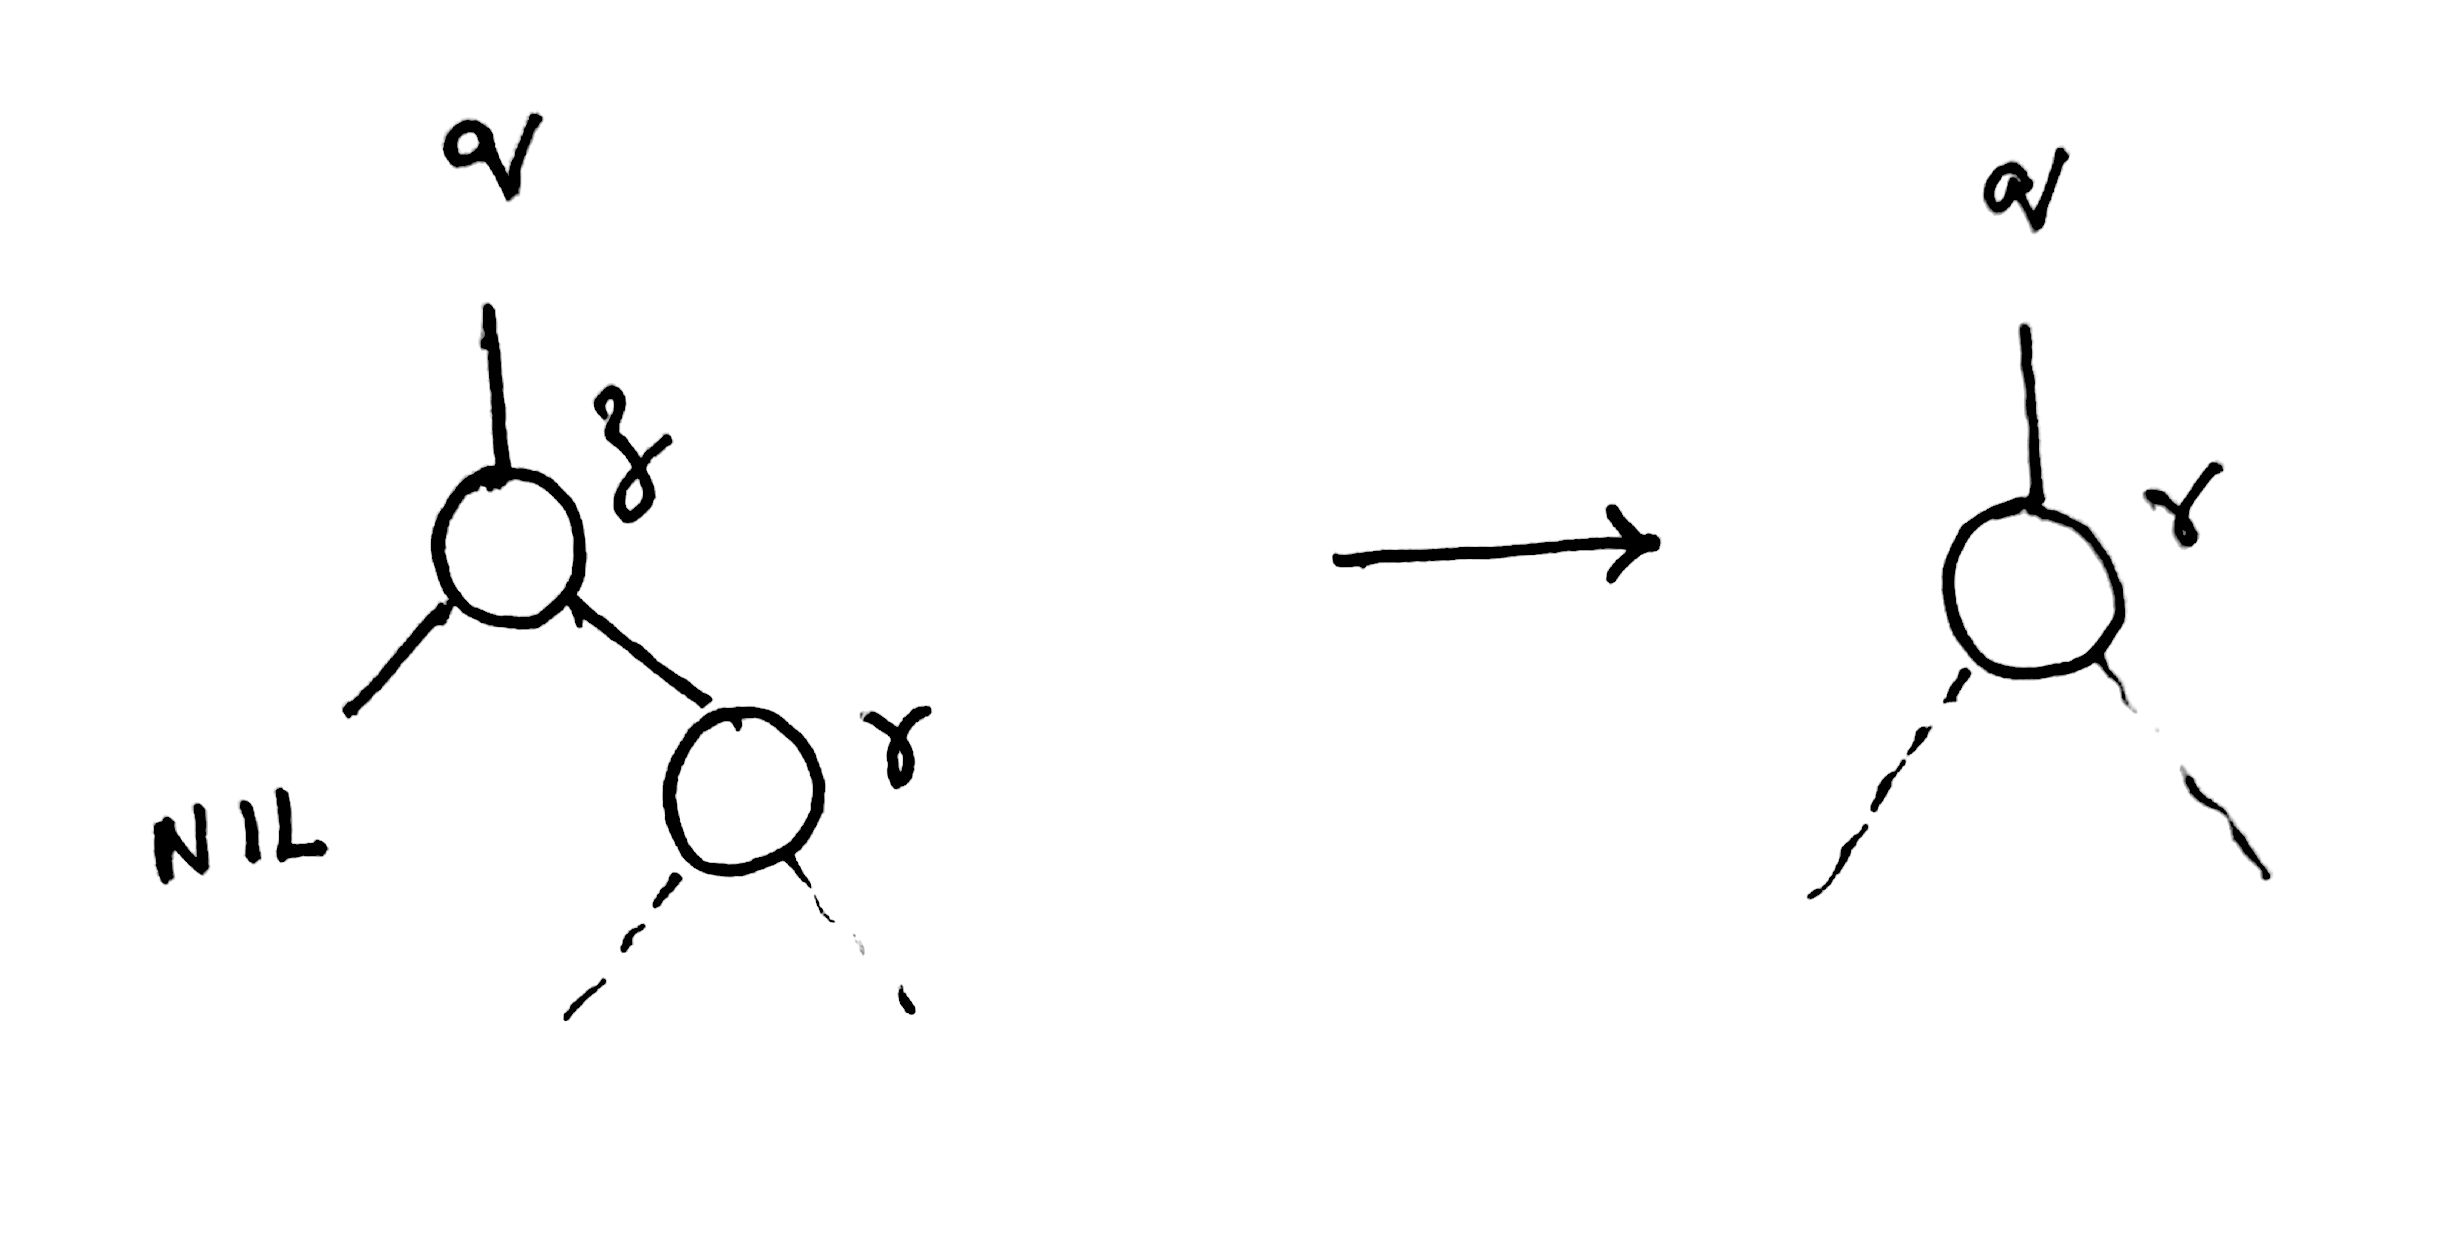
\includegraphics[width=0.5\columnwidth]{a.jpg}
	\label{1}
\end{figure}

\item Node $z$ has a left child $l$ but no right child. We replace $z$ by $l$. This takes only $O(1)$ time
\begin{figure}[H]
	\centering
	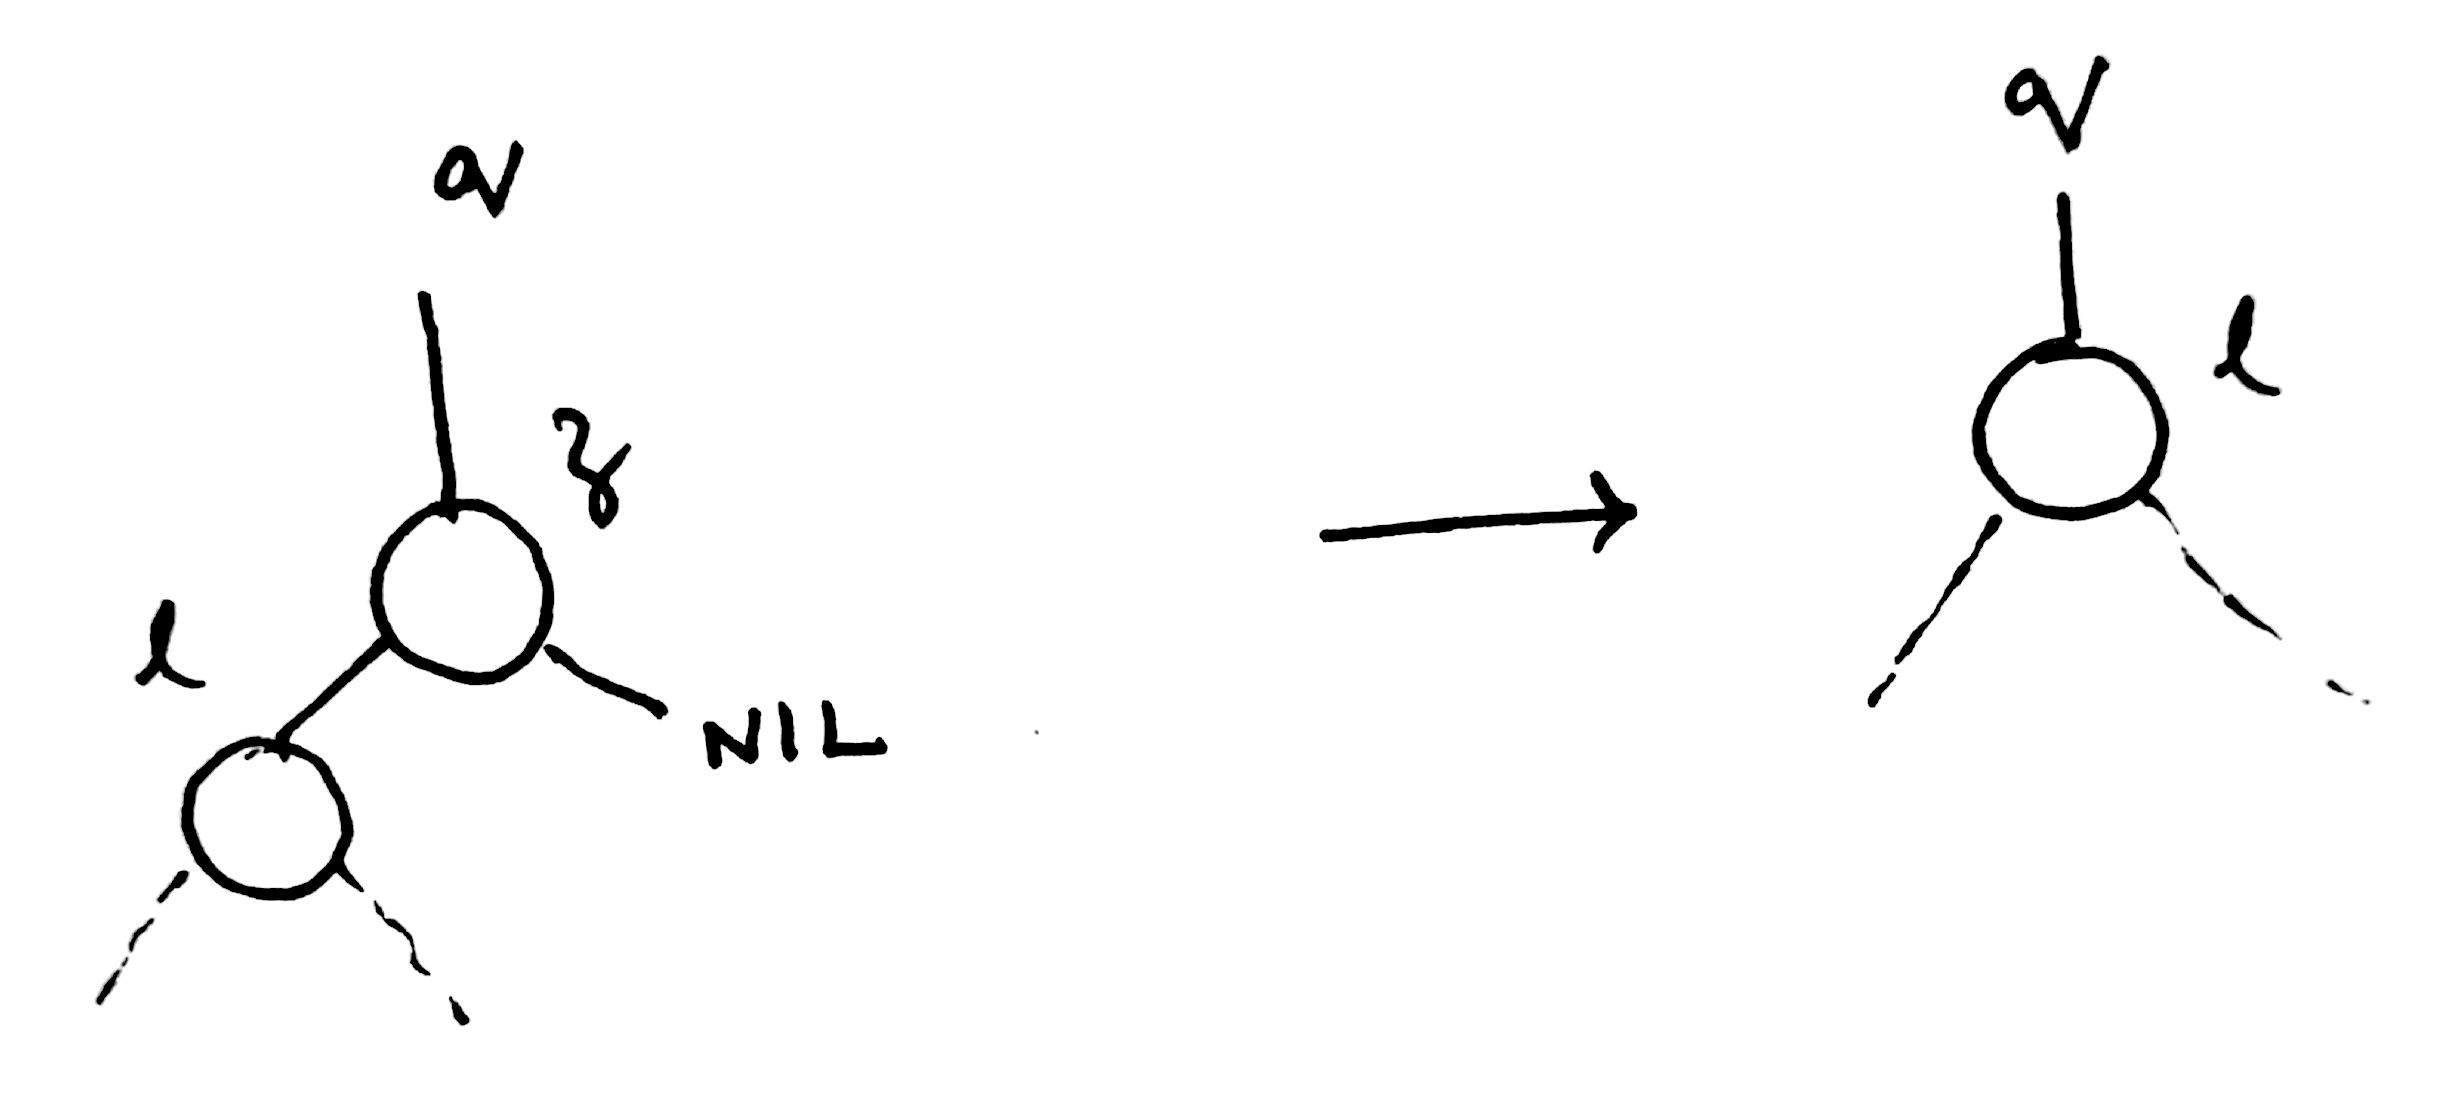
\includegraphics[width=0.5\columnwidth]{b.jpg}
	\label{1}
\end{figure}
\pagebreak
\item Node $z$ has two children, its left child is node $l$, its right child is its successor $y$  and $y$'s right child is node $x$. We replace $z$ by $y$, updating $y$'s left child to become $l$, but leaving $x$ as $y$'s right child and update $even(y) = even(y)+even(l)$. This takes only $O(1)$ time
\begin{figure}[H]
	\centering
	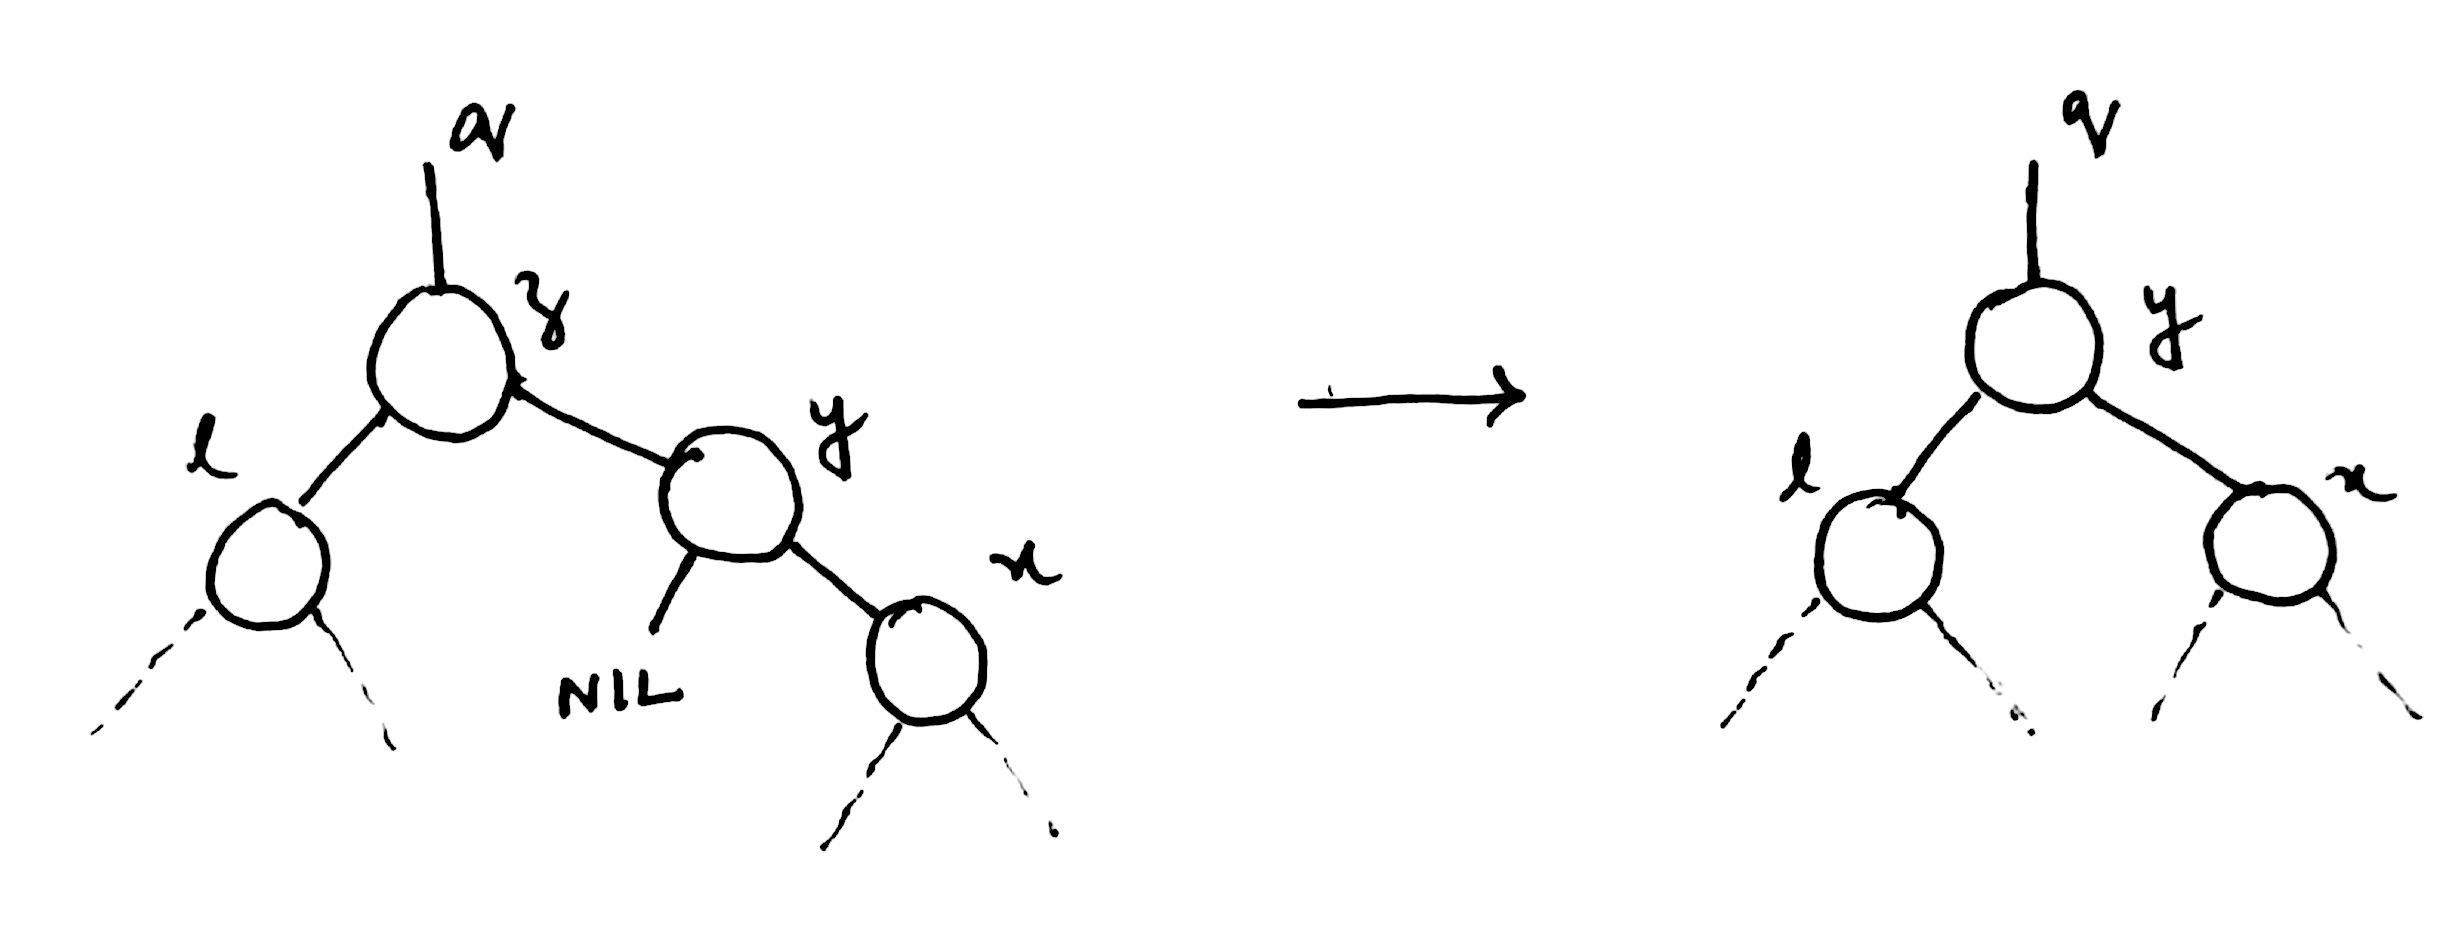
\includegraphics[width=0.65\columnwidth]{c.jpg}
	\label{1}
\end{figure}
update $even(y) = even(y) + even(l)$. Therefore, this takes $O(h)$ time
\item Node $z$
has two children (left child $l$ and right child $r$), and its successor $y \neq r$ lies within the subtree rooted at $r$. If $y$ is even then for each node $u$ starting from $y.p$ to $r$ decrease $even(u)$ by 1 and replace $y$ by it's own right child $x$, set $y$ to be $r$'s parent and update $even(y) = 1+ even(r)$.
\begin{figure}[H]
	\centering
	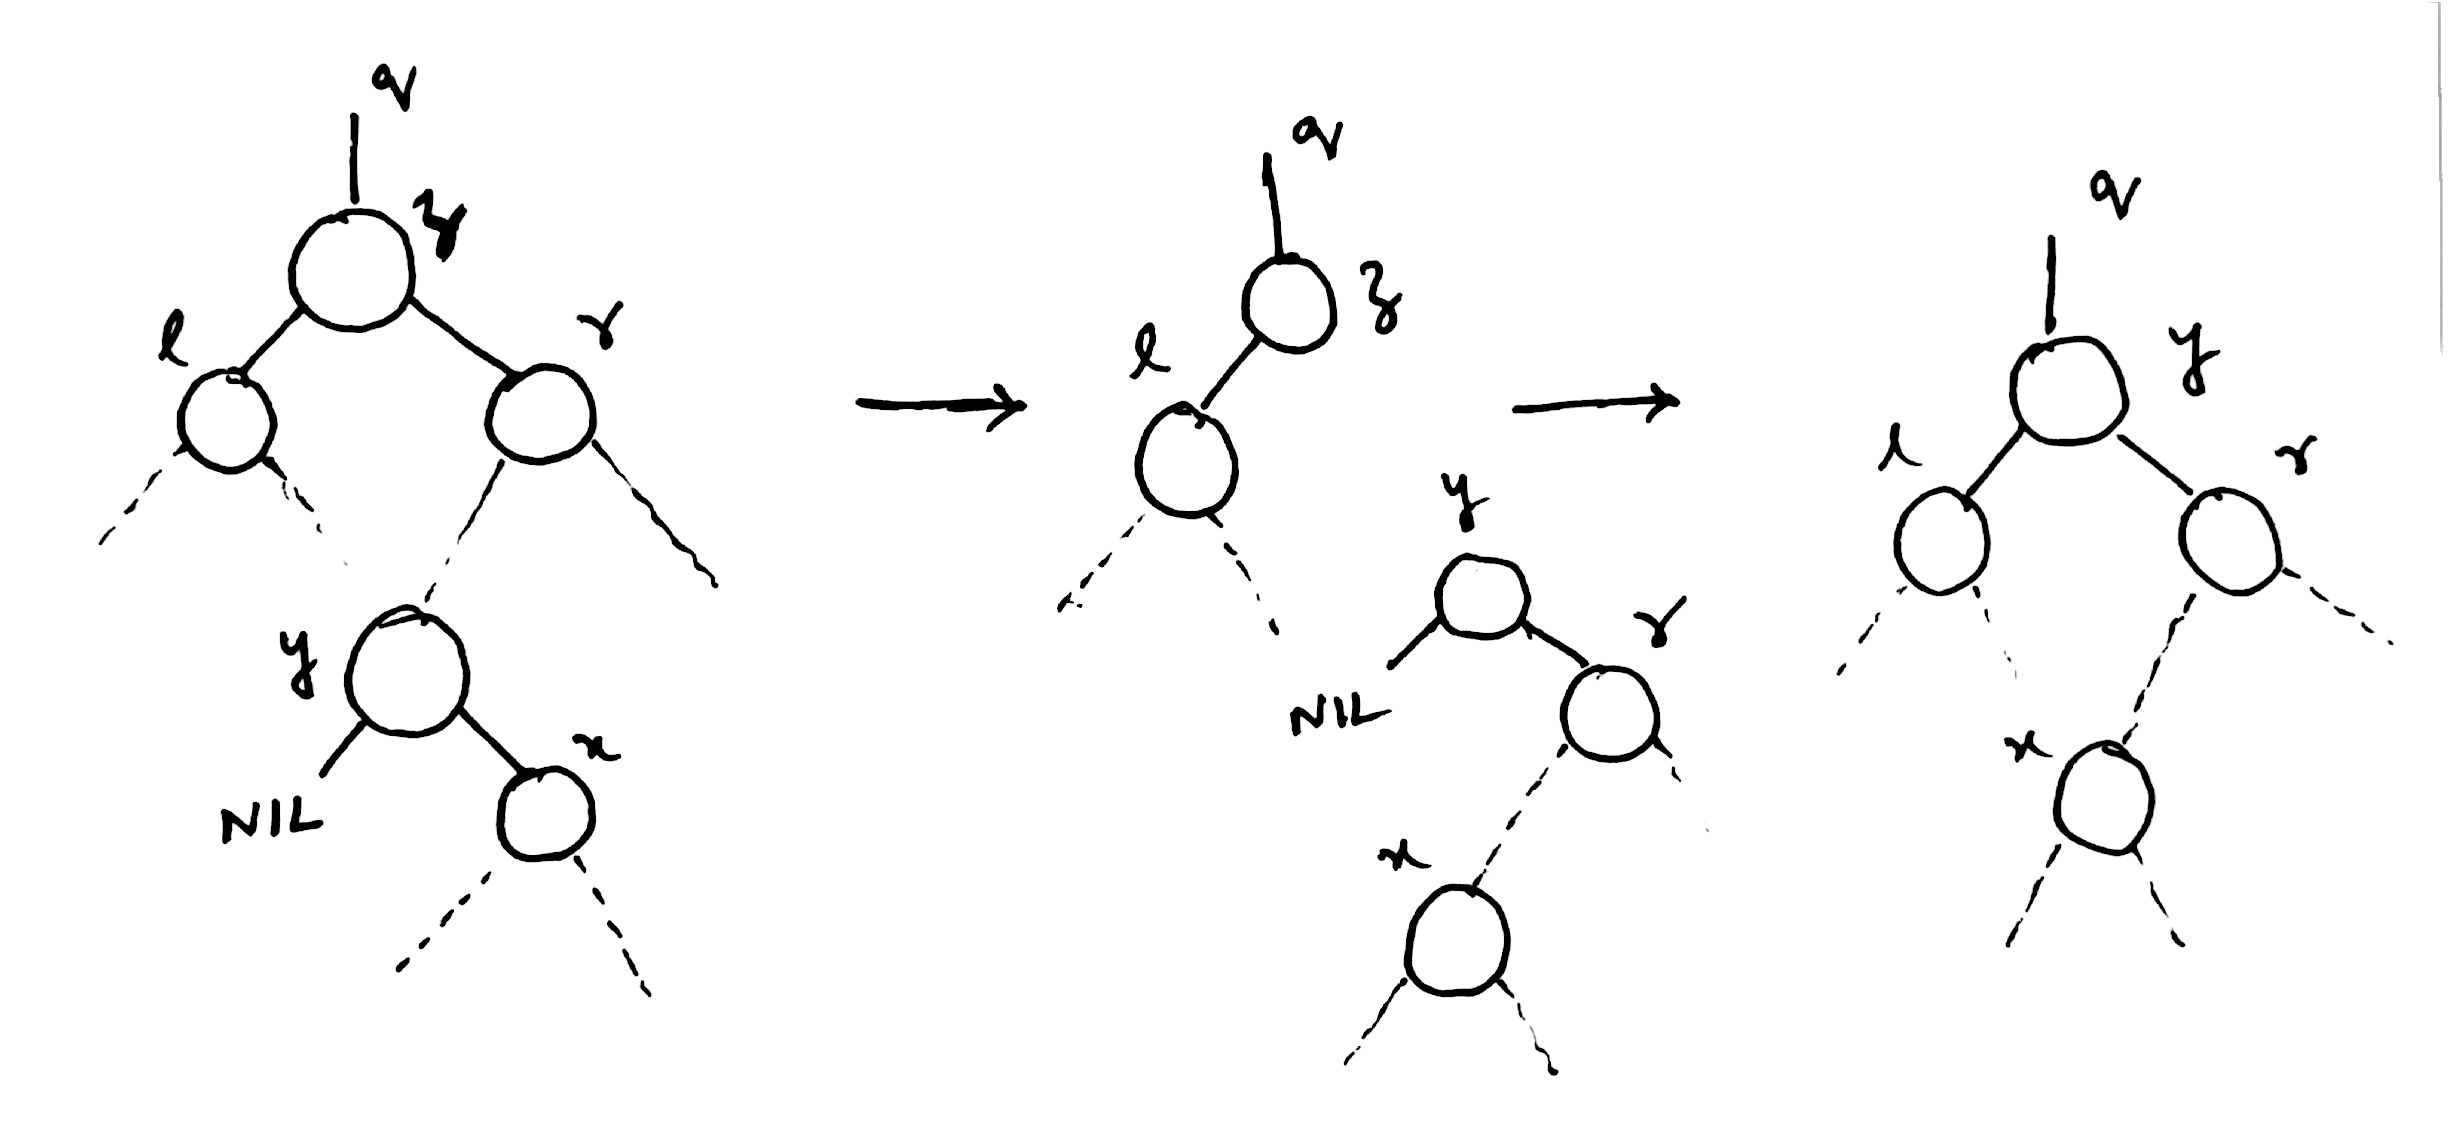
\includegraphics[width=0.8\columnwidth]{d.jpg}
	\label{1}
\end{figure}


Then set $y$ to be $q$'s child and again update $even(y) = even(y) + even(l)$. This, takes $O(h)$ time
\end{itemize}
Therefore by adding some extra computations which take $O(h)$ time we can still perform the delete operation while correctly maintaining the $even(v)$ values in $O(h)$ time
\end{solution}
\fi
\end{itemize}

\newproblem{Matrix Operations} {8 points}

We want to build a data structure for maintaining a (potentially infinite) matrix $M$ and support the following operations.
\begin{itemize}
\item {\sc Initialize}($M$): Create an empty matrix $M$ with all zero entries.
\item {\sc Find}($M,i, j$): Return the value at index $i, j$.
\item {\sc Update}($M, i, j, e$): Change the value at index $i, j$ to $e$.
\item {\sc Transpose}($M$): Transpose the matrix $M$.
\item {\sc Add}($M$): Return the sum of all entries of $M$.
\end{itemize}
Assume that the matrix is of arbitrary dimensions. Use 2-3 trees appropriately to obtain a data structure such that {\sc Initialize}, {\sc Transpose}, and {\sc Add} run in $O(1)$ time, and {\sc Find} and {\sc Update} run in $O(\log k)$ time, where $k$ is the number of non-zero entries in the matrix.

\ifnum\me<2
\begin{solution}

\subsection*{Building \textit{M} using 2-3 Tree}
Let $H$ be a hash function such that $H[(i,j)]$ produces a unique key for each pair $(i,j)$. Assume that applying $H$ on any index $(i,j)$ takes only $O(1)$ time. $\vspace{5pt}$

Let $M$ be an empty 2-3 Tree. Every node $v \in M$ has the following fields
\begin{itemize}
\item $v.left, v.mid, v.right$
\item If $v$ is a leaf node then $v.key$ stores the hashed value of $(i,j)$. If $v$ is a non-leaf node then $v.key$ stores the maximum key of it's children
\item $v.sum$ stores the sum of all the sums of it's children. If $v$ is a leaf node then $v.sum = v.key$
\item If $v$ is a root node then $v$ has one additional field $init$ such that $v.init = k$ initializes all the matrix entries to $k$
\item If $v$ is a leaf node then $v$ has one additional field $value$ where $v.value$ stores the value at $M(i,j)$
\end{itemize}
Now compute $H[(i,j)]$ for every $(i,j)$  and insert them into $M$ while maintaining the above fields at every node.
\pagebreak
\subsection*{{\sc Initialize}($M$)}
Let $x$ be the root of $M$. Update $x.init$ to 0. Therefore, {\sc Initialize} takes $O(1)$ time
\subsection*{{\sc Find}($M,i,j$)}
Compute $H(i,j)$. Now perform the usual Search operation and return $v.value$ where $v$ is the leaf node returned by the Search operation. Therefore, {\sc Find} takes $O(\log k)$ time
\subsection*{{\sc Update}($M, i, j, e$)}
Compute $H(i,j)$. Now perform the usual Search operation and update $v.value$ to $e$ where $v$ is the leaf node returned by the Search operation. Therefore, {\sc Update} takes $O(\log k)$ time
\subsection*{{\sc Transpose}($M$)}
When a matrix is transposed, the indices are all flipped i.e $(i,j) = (j,i)$. Therefore to return any element at $(i,j)$ position return the element at $(j,i)$ position. Therefore, {\sc Transpose} takes $O(1)$ time
\subsection*{{\sc Add}($M$)}
If $x$ is the root of $M$ then return $x.sum$. Therefore, {\sc Add} takes $O(1)$ time
\end{solution}
\fi

\newproblem{Successor of an Element} {14 points}



Assume that you are given a 2-3 tree $T$ containing $n$ distinct elements.

\begin{itemize}
\item[(a)] (4 points) Show how to find the successor of a given
  element $x \in T$ in time $O(\log n)$.

\ifnum\me<2
\begin{solution}

The leaves of 2-3 Trees are in a sorted order when seen from left to the right. Therefore the successor of any given node is the adjacent leaf node to it's right. In order to find the successor of any leaf node $x$, we proceed as follows.
\begin{itemize}
\item Go up the tree to the first ancestor of $x$ that has a child to the right. (i.e we find the first ancestor of $x$, such that the sub tree in which $x$ is located has a right sibling)
\item Find the leftmost leaf node in this sibling sub tree by following the left children all way until the leaf. This leaf we find is the successor of $x$
\end{itemize}
In the worst case, we start from $x$ and go up the tree until the root and then till the bottom to the minimal leaf node in root's right subtree. Therefore, the worst case running time is $O(\log n)$

\end{solution}
\fi

\item[(b)] (4 points) Show that if the input element $x$ is chosen
  {\em uniformly at random} from $T$, then your procedure from part
  (a) runs in {\em expected} time  $O(1)$.

\ifnum\me<2
\begin{solution}

Consider a node $v$ which has three children $a, b$ and $c$. Therefore, $succ(a) = b$ and $succ(b) = c$. Finding the successors of these two nodes takes only $O(1)$ time and to find $succ(c)$ we need to go up the tree until we find an ancestor such that it has a right child. This might take $O(\log n)$ time. Therefore, the probability that the successor operation takes only $O(1)$ time is 2/3 and $O(\log n)$ is 1/3.

 If the node $v$ only two children $a$ and $b$ then it is clear that the probability that the successor operation takes only $O(1)$ time is 1/2 and $O(\log n)$ is 1/2. Therefore, in the worst-case scenario, every node of the tree has only 2 children i.e a perfectly balanced binary tree


Let $n$ be the total number of leaf nodes and $h$ be the height of the 2-3 Tree i.e $h = \log n$

The number of leaf nodes $x$ such that ancestor of $x$ has a right child at height 1 from $x$ is $n/2$. Therefore, finding successor of these $n/2$ nodes takes time $n/2.O(1)$

The number of leaf nodes $x$ such that ancestor of $x$ has a right child at height 2 from $x$ is $n/4$. Therefore, finding successor of these $n/4$ nodes takes time $n/4.O(2)$

The number of leaf nodes $x$ such that ancestor of $x$ has a right child at height 3 from $x$ is $n/8$. Therefore, finding successor of these $n/4$ nodes takes time $n/8.O(3)$

\begin{center}
$\vdots$\\
\end{center}

The number of leaf nodes $x$ such that ancestor of $x$ has a right child at height $\log n$ from $x$ is $1$. Therefore, finding successor of this $1$ node takes time $O(\log n)$

Let $T(n)$ be the expected running time, then

\begin{align*}
T(n) &= \frac{1}{n}[\frac{n}{2} O(1) + \frac{n}{4} O(2) + \frac{n}{8} O(3) + \ldots + 1.O(\log n)]\\
&= \frac{1}{n} \sum_{i = 1}^{\log n} \frac{n}{2^i}O(i)\\
&= \sum_{i = 1}^{\log n} \frac{O(i)}{2^i}
\end{align*}
Consider the summation, $\sum_{i=0}^{\infty} x^j = \frac{1}{1-x}$

Take derivative on both sides and multiply by $x$ we get $\sum_{i=0}^{\infty} ix^i = \frac{x}{(1-x)^2}$

Put $x = 1/2$ in  the above equation, we get $\sum_{i=0}^{\infty} \frac{i}{2^i} = 2 \implies \sum_{i=0}^{\infty} \frac{O(i)}{2^i} = O(1)$
\begin{align*}
T(n) &= \sum_{i = 1}^{\log n} \frac{O(i)}{2^i} \leq \sum_{i=0}^{\infty} \frac{O(i)}{2^i} \\
\therefore T(n) &= O(1)
\end{align*}
\end{solution}
\fi

\end{itemize}

Assume that we wish to augment our 2-3 tree data structure so that
that each node $v$ maintains a pointer $v.succ$ to the successor of
$v$, so that queries for the successor of an element can be answered
in $O(1)$ time {\em worst-case}.

\begin{itemize}
\item[(c)] (6 points) Show that the 2-3 trees can be augmented while
  maintaining $v.succ$, such that the {\sc Insert} and {\sc Delete}
  operations can still be performed in $O(\log n)$ time.
\hint{Think of a linked list.}

 \ifnum\me<2
\begin{solution}

Given that leaf node $v$ has a pointer $v.succ$ to the successor of $v$, so the leaf nodes of the 2-3 Tree form a sorted liked list. 
\subsection*{{\sc Insert}}
Let $y$ be the node to be inserted into the tree. Perform the usual Insert operation in $O(\log n)$ time. 
\begin{itemize}
\item If $y$ is the leftmost leaf node in the tree. Let $z$ be the adjacent leaf node of $y$ to it's right, then $y.succ = z$. This takes $O(1)$ time
\item If $y$ is the rightmost leaf node in the tree. Let $z$ be the adjacent lead node to $y$ to it's left, then $z.succ = y$ and $y.succ = null$. This takes $O(1)$ time
\item Else, Let $x$ be the predecessor of $y$ and let $z$ be $x.succ$ then $x.succ = y$ and $y.succ = z$. This step takes $O(\log n)$ time
\end{itemize}
Therefore, the Insert operation still takes $O(\log n)$ time while maintaining the $succ$ field
\subsection*{{\sc Delete}}
Let $y$ be the node to be deleted in the tree
\begin{itemize}
\item If $y$ is the leftmost or the rightmost leaf node to be deleted in the tree, then perform the usual Delete operation. This step takes $O(\log n)$ time
\item Else, Let $x$ be the predecessor of $y$ and $y.succ$ be $z$, then perform the usual Delete operation and update $x.succ$ to $z$. This step takes $O(\log n)$ time
\end{itemize}
Therefore, the Delete operation still takes $O(\log n)$ time while maintaining the $succ$ field
\end{solution}
\fi

\end{itemize}
\end{document}


